Refer to Example 6.1.
\begin{enumerate}[label= (\alph*)]
    \item Redo the analysis in Example 6.1 after transforming the pairs of observations to $\ln(\text{BOD})$ and $\ln(\text{SS})$.

    \[
        \bar{d}_{1}
        =
        \frac{ \sum_{j=1}^{n}{ d_{j1} } }{n-1}
        =
        \frac{-6.140146}{11}
        =
        -12
    \]
    \[
        \bar{d}_{2}
        =
        \frac{ \sum_{j=1}^{n}{ d_{j2} } }{n-1}
        =
        \frac{3.250811}{11}
        =
        8.6
    \]
    \[
        s_{d_{1}}^{2}
        =
        \frac{ \sum_{j=1}^{n}{( d_{j1} - \bar{d}_{1} )}^{2} }{n-1}
        =
        \frac{1228}{10 - 1}
        =
        0.456081
    \]
    \[
        s_{d_{2}}^{2}
        =
        \frac{ \sum_{j=1}^{n}{( d_{j2} - \bar{d}_{2} )}^{2} }{n-1}
        =
        \frac{1784.4}{10 - 1}
        =
        0.183868
    \]

    \begin{align*}
        H_{0}: & \underset{p \times 1}{\bm{\delta}} = \underset{p \times 1}{\textbf{0}} \\
        H_{a}: & \underset{p \times 1}{\bm{\delta}} \ne \underset{p \times 1}{\textbf{0}}
    \end{align*}

    \[
        \underset{2 \times 1}{\bm{\delta}}
        =
        \left[
            \begin{array}{c}
                \delta_{1} \\
                \delta_{2}
            \end{array}
        \right]
        =
        \left[
            \begin{array}{c}
                {\scriptstyle \ln \left( \text{Commercial lab BOD} \right) - \ln \left( \text{State lab of hygiene BOD} \right)} \\
                {\scriptstyle
                \ln \left( \text{Commercial lab SS} \right) - \ln \left( \text{State lab of hygiene SS} \right)}
            \end{array}
        \right]
    \]

    \[
        T^{2}
        =
        n
        {(\bar{\textbf{d}} - \bm{\delta})}^{\prime}
        \textbf{S}_{d}^{-1}
        (\bar{\textbf{d}} - \bm{\delta})
        =
        n
        {(\bar{\textbf{d}} - \textbf{0})}^{\prime}
        \textbf{S}_{d}^{-1}
        (\bar{\textbf{d}} - \textbf{0})
        =
        n
        {\bar{\textbf{d}}}^{\prime}
        \textbf{S}_{d}^{-1}
        \bar{\textbf{d}}
        =
        10.2154
    \]

    \begin{align*}
        F_{\text{crit}}
        &=
        \frac{(n-1)p}{(n-p)}
        F_{p, n-p}(\alpha) \\
        &=
        \frac{(11-1)2}{(11-2)}
        F_{2, 11-2}(0.05) \\
        &=
        2.22(4.2565) \\
        &=
        9.458877
    \end{align*}
    We have that $T^2 =10.215>F_{\text{crit}} = \frac{10(2)}{9} F_{2,9}(0.05)=9.459$, so we would reject the null hypothesis that $\bm{\delta}=\textbf{0}$.
    Now, to compute the simultaneous 95\% confidence intervals
    \[
        \delta_{1}:
        \bar{d}_{1}
        \pm
        \sqrt{\frac{(n-1)p}{(n-p)}
              F_{p, n-p}(\alpha)}
        \sqrt{ \frac{ s_{d_{1}}^{2} }{n} }
        =
    \]
    \[
        =
        -0.5582
        \pm
        \sqrt{9.4589}
        \sqrt{ \frac{ 0.4561 }{ 11 } }
        \hspace{0.4cm}\text{or}\hspace{0.4cm}
        (-1.1844, 0.0681)
    \]
    To get the original scale, take the exponential of this, and we have
    \[
        (e^{-1.1844}, ^{0.0681})
        =
        (0.3059, 1.0704)
    \]
    \[
        \delta_{2}:
        \bar{d}_{2}
        \pm
        \sqrt{\frac{(n-1)p}{(n-p)}
              F_{p, n-p}(\alpha)}
        \sqrt{ \frac{ s_{d_{2}}^{2} }{n} }
        =
    \]
    \[
        =
        0.2955
        \pm
        \sqrt{9.4589}
        \sqrt{ \frac{ 0.1839 }{ 11 } }
        \hspace{0.4cm}\text{or}\hspace{0.4cm}
        (-0.1021, 0.6932)
    \]
    To get the original scale, take the exponential of this, and we have
    \[
        (e^{-0.1021}, e^{0.6932})
        =
        (0.9029, 2.0000)
    \]

    \item Construct the 95\% Bonferroni simultaneous intervals for the components of the
    mean vector $\bm{\delta}$ of transformed variables.

    \[
        t_{n-1}(\alpha/2p)
        =
        t_{11-1}(0.05/[2(2)])
        =
        2.633767
    \]
    \[
        \delta_{1}:
        \bar{d}_{1}
        \pm
        t_{n - 1}(\alpha/2p)
        \sqrt{ \frac{ s_{d_{1}}^{2} }{n} }
        =
    \]
    \[
        =
        -0.5582
        \pm
        2.6338
        \sqrt{ \frac{ 0.4561 }{ 11 } }
        \hspace{0.4cm}\text{or}\hspace{0.4cm}
        (-1.0945, -0.0219)
    \]
    To get the original scale, take the exponential of this, and we have
    \[
        (e^{-1.0945}, ^{-0.0219})
        =
        (0.3347, 0.9783)
    \]
    \[
        \delta_{2}:
        \bar{d}_{2}
        \pm
        t_{n - 1}(\alpha/2p)
        \sqrt{ \frac{ s_{d_{2}}^{2} }{n} }
        =
    \]
    \[
        =
        0.2955
        \pm
        2.6338
        \sqrt{ \frac{ 0.1839 }{ 11 } }
        \hspace{0.4cm}\text{or}\hspace{0.4cm}
        (-0.0450, 0.6360)
    \]
    To get the original scale, take the exponential of this, and we have
    \[
        (e^{-0.0450}, e^{0.6360})
        =
        (0.9560, 1.8890)
    \]

    \item Discuss any possible violation of the assumption of a bivariate normal distribution
    for the difference vectors of transformed observations.

    \begin{figure}[H]
        \centering
        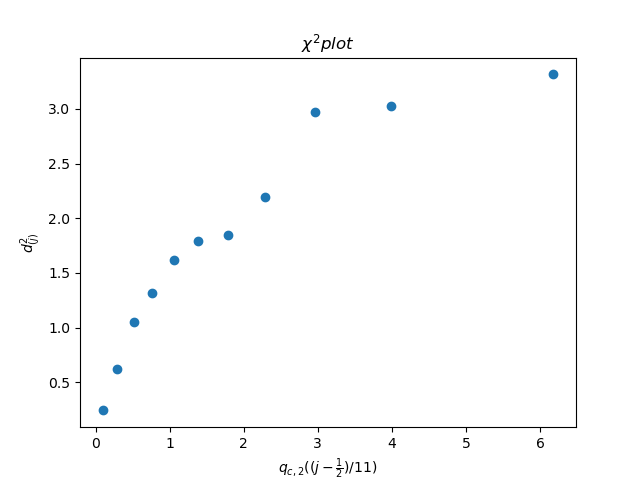
\includegraphics[scale=0.70]{./python/chapter-6/Question-6-4-c.png}
    \end{figure}

    Using the tools in Chapter 4, on pages 182 and 183, by computing the generalized squared distances and comparing them to the 50\% contour, we'd expect 50\% of the data to be within the contour. For this data, actually 100\% is within the contour. This isn't a good sign.
    Also creating a $\chi^{2}$-plot, seen above, it should appear linear. However, a quick glance reveals that's not the case. I'd conclude, based on these two things, that the data is not normally distributed after a $\ln$ transformation.

\end{enumerate}